
%% bare_conf_compsoc.tex
%% V1.4b
%% 2015/08/26
%% by Michael Shell
%% See:
%% http://www.michaelshell.org/
%% for current contact information.
%%
%% This is a skeleton file demonstrating the use of IEEEtran.cls
%% (requires IEEEtran.cls version 1.8b or later) with an IEEE Computer
%% Society conference paper.
%%
%% Support sites:
%% http://www.michaelshell.org/tex/ieeetran/
%% http://www.ctan.org/pkg/ieeetran
%% and
%% http://www.ieee.org/

%%*************************************************************************
%% Legal Notice:
%% This code is offered as-is without any warranty either expressed or
%% implied; without even the implied warranty of MERCHANTABILITY or
%% FITNESS FOR A PARTICULAR PURPOSE! 
%% User assumes all risk.
%% In no event shall the IEEE or any contributor to this code be liable for
%% any damages or losses, including, but not limited to, incidental,
%% consequential, or any other damages, resulting from the use or misuse
%% of any information contained here.
%%
%% All comments are the opinions of their respective authors and are not
%% necessarily endorsed by the IEEE.
%%
%% This work is distributed under the LaTeX Project Public License (LPPL)
%% ( http://www.latex-project.org/ ) version 1.3, and may be freely used,
%% distributed and modified. A copy of the LPPL, version 1.3, is included
%% in the base LaTeX documentation of all distributions of LaTeX released
%% 2003/12/01 or later.
%% Retain all contribution notices and credits.
%% ** Modified files should be clearly indicated as such, including  **
%% ** renaming them and changing author support contact information. **
%%*************************************************************************


% *** Authors should verify (and, if needed, correct) their LaTeX system  ***
% *** with the testflow diagnostic prior to trusting their LaTeX platform ***
% *** with production work. The IEEE's font choices and paper sizes can   ***
% *** trigger bugs that do not appear when using other class files.       ***                          ***
% The testflow support page is at:
% http://www.michaelshell.org/tex/testflow/



\documentclass[conference,compsoc]{IEEEtran}
% Some/most Computer Society conferences require the compsoc mode option,
% but others may want the standard conference format.
%
% If IEEEtran.cls has not been installed into the LaTeX system files,
% manually specify the path to it like:
% \documentclass[conference,compsoc]{../sty/IEEEtran}





% Some very useful LaTeX packages include:
% (uncomment the ones you want to load)


\usepackage{graphicx}
% *** MISC UTILITY PACKAGES ***
%
%\usepackage{ifpdf}
% Heiko Oberdiek's ifpdf.sty is very useful if you need conditional
% compilation based on whether the output is pdf or dvi.
% usage:
% \ifpdf
%   % pdf code
% \else
%   % dvi code
% \fi
% The latest version of ifpdf.sty can be obtained from:
% http://www.ctan.org/pkg/ifpdf
% Also, note that IEEEtran.cls V1.7 and later provides a builtin
% \ifCLASSINFOpdf conditional that works the same way.
% When switching from latex to pdflatex and vice-versa, the compiler may
% have to be run twice to clear warning/error messages.






% *** CITATION PACKAGES ***
%
\ifCLASSOPTIONcompsoc
  % IEEE Computer Society needs nocompress option
  % requires cite.sty v4.0 or later (November 2003)
  \usepackage[nocompress]{cite}
\else
  % normal IEEE
  \usepackage{cite}
\fi
% cite.sty was written by Donald Arseneau
% V1.6 and later of IEEEtran pre-defines the format of the cite.sty package
% \cite{} output to follow that of the IEEE. Loading the cite package will
% result in citation numbers being automatically sorted and properly
% "compressed/ranged". e.g., [1], [9], [2], [7], [5], [6] without using
% cite.sty will become [1], [2], [5]--[7], [9] using cite.sty. cite.sty's
% \cite will automatically add leading space, if needed. Use cite.sty's
% noadjust option (cite.sty V3.8 and later) if you want to turn this off
% such as if a citation ever needs to be enclosed in parenthesis.
% cite.sty is already installed on most LaTeX systems. Be sure and use
% version 5.0 (2009-03-20) and later if using hyperref.sty.
% The latest version can be obtained at:
% http://www.ctan.org/pkg/cite
% The documentation is contained in the cite.sty file itself.
%
% Note that some packages require special options to format as the Computer
% Society requires. In particular, Computer Society  papers do not use
% compressed citation ranges as is done in typical IEEE papers
% (e.g., [1]-[4]). Instead, they list every citation separately in order
% (e.g., [1], [2], [3], [4]). To get the latter we need to load the cite
% package with the nocompress option which is supported by cite.sty v4.0
% and later.





% *** GRAPHICS RELATED PACKAGES ***
%
\ifCLASSINFOpdf
  % \usepackage[pdftex]{graphicx}
  % declare the path(s) where your graphic files are
  % \graphicspath{{../pdf/}{../jpeg/}}
  % and their extensions so you won't have to specify these with
  % every instance of \includegraphics
  % \DeclareGraphicsExtensions{.pdf,.jpeg,.png}
\else
  % or other class option (dvipsone, dvipdf, if not using dvips). graphicx
  % will default to the driver specified in the system graphics.cfg if no
  % driver is specified.
  % \usepackage[dvips]{graphicx}
  % declare the path(s) where your graphic files are
  % \graphicspath{{../eps/}}
  % and their extensions so you won't have to specify these with
  % every instance of \includegraphics
  % \DeclareGraphicsExtensions{.eps}
\fi
% graphicx was written by David Carlisle and Sebastian Rahtz. It is
% required if you want graphics, photos, etc. graphicx.sty is already
% installed on most LaTeX systems. The latest version and documentation
% can be obtained at: 
% http://www.ctan.org/pkg/graphicx
% Another good source of documentation is "Using Imported Graphics in
% LaTeX2e" by Keith Reckdahl which can be found at:
% http://www.ctan.org/pkg/epslatex
%
% latex, and pdflatex in dvi mode, support graphics in encapsulated
% postscript (.eps) format. pdflatex in pdf mode supports graphics
% in .pdf, .jpeg, .png and .mps (metapost) formats. Users should ensure
% that all non-photo figures use a vector format (.eps, .pdf, .mps) and
% not a bitmapped formats (.jpeg, .png). The IEEE frowns on bitmapped formats
% which can result in "jaggedy"/blurry rendering of lines and letters as
% well as large increases in file sizes.
%
% You can find documentation about the pdfTeX application at:
% http://www.tug.org/applications/pdftex





% *** MATH PACKAGES ***
%
%\usepackage{amsmath}
% A popular package from the American Mathematical Society that provides
% many useful and powerful commands for dealing with mathematics.
%
% Note that the amsmath package sets \interdisplaylinepenalty to 10000
% thus preventing page breaks from occurring within multiline equations. Use:
%\interdisplaylinepenalty=2500
% after loading amsmath to restore such page breaks as IEEEtran.cls normally
% does. amsmath.sty is already installed on most LaTeX systems. The latest
% version and documentation can be obtained at:
% http://www.ctan.org/pkg/amsmath





% *** SPECIALIZED LIST PACKAGES ***
%
%\usepackage{algorithmic}
% algorithmic.sty was written by Peter Williams and Rogerio Brito.
% This package provides an algorithmic environment fo describing algorithms.
% You can use the algorithmic environment in-text or within a figure
% environment to provide for a floating algorithm. Do NOT use the algorithm
% floating environment provided by algorithm.sty (by the same authors) or
% algorithm2e.sty (by Christophe Fiorio) as the IEEE does not use dedicated
% algorithm float types and packages that provide these will not provide
% correct IEEE style captions. The latest version and documentation of
% algorithmic.sty can be obtained at:
% http://www.ctan.org/pkg/algorithms
% Also of interest may be the (relatively newer and more customizable)
% algorithmicx.sty package by Szasz Janos:
% http://www.ctan.org/pkg/algorithmicx




% *** ALIGNMENT PACKAGES ***
%
%\usepackage{array}
% Frank Mittelbach's and David Carlisle's array.sty patches and improves
% the standard LaTeX2e array and tabular environments to provide better
% appearance and additional user controls. As the default LaTeX2e table
% generation code is lacking to the point of almost being broken with
% respect to the quality of the end results, all users are strongly
% advised to use an enhanced (at the very least that provided by array.sty)
% set of table tools. array.sty is already installed on most systems. The
% latest version and documentation can be obtained at:
% http://www.ctan.org/pkg/array


% IEEEtran contains the IEEEeqnarray family of commands that can be used to
% generate multiline equations as well as matrices, tables, etc., of high
% quality.




% *** SUBFIGURE PACKAGES ***
%\ifCLASSOPTIONcompsoc
%  \usepackage[caption=false,font=footnotesize,labelfont=sf,textfont=sf]{subfig}
%\else
%  \usepackage[caption=false,font=footnotesize]{subfig}
%\fi
% subfig.sty, written by Steven Douglas Cochran, is the modern replacement
% for subfigure.sty, the latter of which is no longer maintained and is
% incompatible with some LaTeX packages including fixltx2e. However,
% subfig.sty requires and automatically loads Axel Sommerfeldt's caption.sty
% which will override IEEEtran.cls' handling of captions and this will result
% in non-IEEE style figure/table captions. To prevent this problem, be sure
% and invoke subfig.sty's "caption=false" package option (available since
% subfig.sty version 1.3, 2005/06/28) as this is will preserve IEEEtran.cls
% handling of captions.
% Note that the Computer Society format requires a sans serif font rather
% than the serif font used in traditional IEEE formatting and thus the need
% to invoke different subfig.sty package options depending on whether
% compsoc mode has been enabled.
%
% The latest version and documentation of subfig.sty can be obtained at:
% http://www.ctan.org/pkg/subfig




% *** FLOAT PACKAGES ***
%
%\usepackage{fixltx2e}
% fixltx2e, the successor to the earlier fix2col.sty, was written by
% Frank Mittelbach and David Carlisle. This package corrects a few problems
% in the LaTeX2e kernel, the most notable of which is that in current
% LaTeX2e releases, the ordering of single and double column floats is not
% guaranteed to be preserved. Thus, an unpatched LaTeX2e can allow a
% single column figure to be placed prior to an earlier double column
% figure.
% Be aware that LaTeX2e kernels dated 2015 and later have fixltx2e.sty's
% corrections already built into the system in which case a warning will
% be issued if an attempt is made to load fixltx2e.sty as it is no longer
% needed.
% The latest version and documentation can be found at:
% http://www.ctan.org/pkg/fixltx2e


%\usepackage{stfloats}
% stfloats.sty was written by Sigitas Tolusis. This package gives LaTeX2e
% the ability to do double column floats at the bottom of the page as well
% as the top. (e.g., "\begin{figure*}[!b]" is not normally possible in
% LaTeX2e). It also provides a command:
%\fnbelowfloat
% to enable the placement of footnotes below bottom floats (the standard
% LaTeX2e kernel puts them above bottom floats). This is an invasive package
% which rewrites many portions of the LaTeX2e float routines. It may not work
% with other packages that modify the LaTeX2e float routines. The latest
% version and documentation can be obtained at:
% http://www.ctan.org/pkg/stfloats
% Do not use the stfloats baselinefloat ability as the IEEE does not allow
% \baselineskip to stretch. Authors submitting work to the IEEE should note
% that the IEEE rarely uses double column equations and that authors should try
% to avoid such use. Do not be tempted to use the cuted.sty or midfloat.sty
% packages (also by Sigitas Tolusis) as the IEEE does not format its papers in
% such ways.
% Do not attempt to use stfloats with fixltx2e as they are incompatible.
% Instead, use Morten Hogholm'a dblfloatfix which combines the features
% of both fixltx2e and stfloats:
%
% \usepackage{dblfloatfix}
% The latest version can be found at:
% http://www.ctan.org/pkg/dblfloatfix




% *** PDF, URL AND HYPERLINK PACKAGES ***
%
%\usepackage{url}
% url.sty was written by Donald Arseneau. It provides better support for
% handling and breaking URLs. url.sty is already installed on most LaTeX
% systems. The latest version and documentation can be obtained at:
% http://www.ctan.org/pkg/url
% Basically, \url{my_url_here}.




% *** Do not adjust lengths that control margins, column widths, etc. ***
% *** Do not use packages that alter fonts (such as pslatex).         ***
% There should be no need to do such things with IEEEtran.cls V1.6 and later.
% (Unless specifically asked to do so by the journal or conference you plan
% to submit to, of course. )


% correct bad hyphenation here
\hyphenation{op-tical net-works semi-conduc-tor}


\begin{document}
%
% paper title
% Titles are generally capitalized except for words such as a, an, and, as,
% at, but, by, for, in, nor, of, on, or, the, to and up, which are usually
% not capitalized unless they are the first or last word of the title.
% Linebreaks \\ can be used within to get better formatting as desired.
% Do not put math or special symbols in the title.
\title{System Design Considerations for Internet of Things (IoT) with category-M devices in LTE networks}


% author names and affiliations
% use a multiple column layout for up to three different
% affiliations
\author{\IEEEauthorblockN{Gurudutt Hosangadi}
\IEEEauthorblockA{Nokia\\
600-700 Mountain Ave,Murray Hill \\
NJ 07974-0636, USA \\
Email:gurudutt.hosangadi@nokia.com}
\and
\IEEEauthorblockN{Dandan Wang}
\IEEEauthorblockA{Nokia\\
600-700 Mountain Ave, Murray Hill \\
NJ 07974-0636, USA \\
Email:dandan.wang@nokia.com}
\and
\IEEEauthorblockN{Anil Rao}
\IEEEauthorblockA{Nokia \\
12004 173rd Pl NE \\
Redmond, WA 98052, USA \\
Email:anil.rao@nokia.com}}

% conference papers do not typically use \thanks and this command
% is locked out in conference mode. If really needed, such as for
% the acknowledgment of grants, issue a \IEEEoverridecommandlockouts
% after \documentclass

% for over three affiliations, or if they all won't fit within the width
% of the page (and note that there is less available width in this regard for
% compsoc conferences compared to traditional conferences), use this
% alternative format:
% 
%\author{\IEEEauthorblockN{Michael Shell\IEEEauthorrefmark{1},
%Homer Simpson\IEEEauthorrefmark{2},
%James Kirk\IEEEauthorrefmark{3}, 
%Montgomery Scott\IEEEauthorrefmark{3} and
%Eldon Tyrell\IEEEauthorrefmark{4}}
%\IEEEauthorblockA{\IEEEauthorrefmark{1}School of Electrical and Computer Engineering\\
%Georgia Institute of Technology,
%Atlanta, Georgia 30332--0250\\ Email: see http://www.michaelshell.org/contact.html}
%\IEEEauthorblockA{\IEEEauthorrefmark{2}Twentieth Century Fox, Springfield, USA\\
%Email: homer@thesimpsons.com}
%\IEEEauthorblockA{\IEEEauthorrefmark{3}Starfleet Academy, San Francisco, California 96678-2391\\
%Telephone: (800) 555--1212, Fax: (888) 555--1212}
%\IEEEauthorblockA{\IEEEauthorrefmark{4}Tyrell Inc., 123 Replicant Street, Los Angeles, California 90210--4321}}




% use for special paper notices
%\IEEEspecialpapernotice{(Invited Paper)}




% make the title area
\maketitle

% As a general rule, do not put math, special symbols or citations
% in the abstract
\begin{abstract}
    Successful network deployment of the Internet of Things (IoT) requires many critical system design considerations. This paper highlights how an LTE system supporting Cat-M devices can be engineered to deal with the numerous constraints the 3GPP standard imposes for this new device type. Fundamental changes to the control channels, control and data timing relationships, the need to support half-duplexing, and variable repetition lengths for both data and control channels pose non-trivial challenges, particularly when attempting to satisfy the critical coverage KPI for Cat-M devices while at the same time preserving the capacity KPI for legacy LTE devices. In addition, the nature of IoT traffic is fundamentally different than legacy LTE data, requiring changes to existing system parameters and MAC algorithms.  Finally, we will touch upon the very recent topic of supporting voice over IP traffic on Cat-M devices and the challenges therin.
\end{abstract}

% no keywords




% For peer review papers, you can put extra information on the cover
% page as needed:
% \ifCLASSOPTIONpeerreview
% \begin{center} \bfseries EDICS Category: 3-BBND \end{center}
% \fi
%
% For peerreview papers, this IEEEtran command inserts a page break and
% creates the second title. It will be ignored for other modes.
\IEEEpeerreviewmaketitle



\section{Introduction}
% no \IEEEPARstart
The internet of things (IoT) buildup is well underway. The number of connected devices worldwide was around 5 billion in 2014 and is expected to reach 50 billion by 2020 [1]. These devices cover a wide range of applications:  wearable devices, connected home appliances, remote sensing for utilities and smart cities to name a few. New applications are being devised daily which rely on the basic philosophy that any device with the ability to connect to the internet can be utilized in a smart way to either improve automation or provide connectivity in very small form factors. These massive number of devices communicating without human intervention constitute to what is commonly called as machine type communication (MTC) or referred to as the Internet of Things (IoT). Modern wireless cellular networks such LTE (Long Term Evolution) based on 3rd Generation Partnership Project (3GPP) are aptly placed to be an enabler of massive MTC. This is due to its all-inclusive-all-IP architecture, built in security, scalable traffic management capabilities and high spectral efficiencies.
The traffic profile and requirement of IoT differs vastly from that of traditional mobile devices already supported in LTE cellular networks. Key differences include smaller traffic packet sizes and massive number of such devices. To support this change, 3GPP standards have been enhanced with new features. See [3.6] for a detailed coverage of the added features.
In this tutorial, we focus on system design considerations of IoT devices. As we will show, the unique characteristics of IoT devices pose challenges to system design.  Also, it is important for  the design to minimize the impact to the key performance indicators (KPIs) of traditional service offerings given that  traditional services and MTC traffic share the same wireless resources. Finally, we present some insights into performance based on our simulation results. For this, we specifically focus on the CaT-M feature within the LTE standards, which some major service providers are considering deploying to enhance their offered services for IoT.

% You must have at least 2 lines in the paragraph with the drop letter
% (should never be an issue)

%\hfill mds
 
%\hfill April 11, 2018 

\section{Requirements}
MTC devices pose a new set of requirements and challenges [2] to system design as shown in Figure 1. First and foremost is that the introduction of a large number MTC devices into the system should have a minimum impact on the operation of legacy devices. Next, MTC devices are expected to be low cost, low complexity, and have low power consumption. These attributes need to be considered in system design. Finally, MTC devices would be useful only if certain performance targets are met. We discuss each of these competing aspects next.

\begin{figure}[htbp]
\centerline{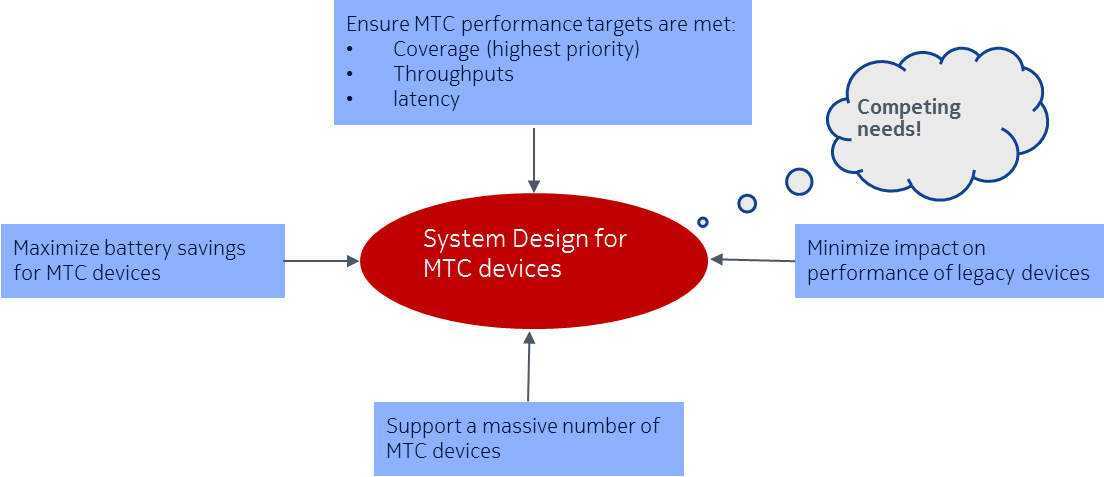
\includegraphics[height=40mm,width=80mm]{sys_design.png}}
\caption{System Design for MTC devices}
\label{fig_sys_design}
\end{figure}

\subsection{MTC Performance Targets}
As illustrated in [3], enhanced coverage is one of the key requirements of   MTC given the targeted application of these devices. The primary mechanisms that have been available in standards to improve coverage prior to Release 13 are hybrid automatic repeat request (HARQ) retransmissions. which primarily improve energy accumulation and can benefit from fading and interference diversity effects in the time domain.  For dramatic improvements in coverage, a very large number of retransmissions will be required; for example, a 20dB coverage improvement would require approximately 100 retransmissions This will consume more uplink control channel resources to feedback acknowledgements (via ACK/NACK) for downlink and extra PDCCH grants as each HARQ retransmission on either uplink or downlink needs an explicit grant. Such a large number of signalling channel transmissions will be prone to errors which may result in soft buffer corruption. Due to the half duplexing nature of the Cat-M devices, the time duration to complete one HARQ round is much longer compared to legacy LTE devices operating in full duplex mode, resulting in large latencies if a large number of HARQ retransmissions were to be used. In addition, the half duplexing makes the scheduling of packets on multiple HARQ processes in parallel more challenging (as explained in later sections), which further reduces the efficiency of HARQ retransmissions and prolongs the time that the UE will need to remain awake in order to transmit or receive a packet.  

Due to the above-mentioned disadvantages of HARQ retransmissions, Rel 13 introduces a mechanism of repetition which is similar to transmission time interval (TTI) bundling in Rel 8 intended for voice over IP (VoIP) packets where consecutive TTIs are used to transmit the same packet. Note that in release 13, the number of repetitions can be as high as 256 while in Rel 8 the number of repetitions was limited to 4. However, a word of caution using repetitions:there is a tradeoffusing repetition versus using HARQ. HARQ provides a potential resource saving since the retransmission of HARQ can be terminated once the packet can be successfully decoded while all the transmission within the same repetition have to be sent unconditionally (as there is no ACK/NACK feedback in the middle of transmission). For example, an MTC device that does not require high coverage may be better served by using a small repetition size along with a combination on HARQ retransmission compared to a cell edge UE which will rely primarily on repetition. 

Another system design tradeoff is between coverage and throughput/latency. While the peak rate is 1 Mbps (as per 3GPP), in reality, the achievable rates could be much lower for typical devices depending on when resources are available, what kind of repetition is used, and the traffic profile of users in the system. In the next section we provide some examples on achievable rates observed in simulations for some sample configurations.

\subsection{Low cost}
This is mainly facilitated by standards which have reduced the operating bandwidth , maximum transmitted power, singlereceive RF chain (only 1 receive antenna is supported) and longer discontinuous reception (DRX) cycles.This is discussed in more detail later.

\subsection{Minimal impact to legacy devices}
A key selling point with the introduction of Cat-M devices in LTE is that it can work seamlessly together with legacy LTE devices on existing spectrum, with only a software upgrade needed for an operator to support Cat-M devices and capitalize on the MTC/IoT device explosion. To support this, 3GPP standards allows a MTC device to monitor and process a narrow bandwidth (1.4MHz for Cat.M1 and 200KHz for Cat.NB1)within the available bandwidth; this is referred to as a “narrowband”. An example of possible narrowbands is shown in Figure 2. One design choice may be to reserve this narrow band for Cat-M devices only while the legacy LTE devices use the rest of the available bandwidth. However, this simple design does not consider the instantaneous resource needs of Cat-M and legacy devices. For example, during a short time window, the reserved narrowband for Cat-M devices may go unused due to the sporadic nature of IoT traffic, while the network is at the same time heavily loaded with traffic from legacy LTE devices. A more comprehensive approach would be to have a unified mechanism to dynamically share the narrow band frequency resources between Cat-M and legacy devices taking into consideration quality of service (QoS) requirements. While designing this unified mechanism, we need to consider the unique constraints of the Cat-M devices, such as thelarge number of repetitions, half-duplexing requirement, and the fact that the grant and data channel cannot coexistent in the same TTI. These differences introduce complexity in the system design

\section{System design}
.   In this section, we will discuss in more detail the different aspects of the system design to support Cat-M devices.

\subsection{Location of Narrowbands}
Of importance is  the location of the narrow bandwidth used for MTC devices and the alignment of this bandwidth with resource block groups (RBGs) which may be used by the scehduler. The objective is to minimize the impact to RBG allocation.  For example, Figure 2 illustrates the location of narrowbands for 10MHz. If we useNB0, then RBG0, RBG1, and RBG2 are all impacted and total 9 PRBs can’t be used for RBG allocation. However, if we use NB7, 8 PRBs (RBG14, RBG15 and RBG16) can’t be used for RBG allocation.

Another consideration is that 3GPP standards allows frequency hopping (during repetition) of the narrowband  to experience gains from frequency diversity. Since the hopping is on resources used by legacy devices, appropriate mechanisms to avoid collisions need to be designed.

\begin{figure}[htbp]
\centerline{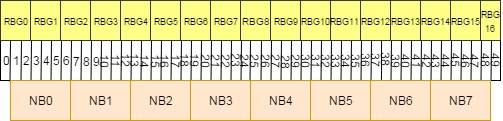
\includegraphics[height=40mm,width=80mm]{narrowband.png}}
\caption{Narrowband illustration}
\label{fig_narrowband}
\end{figure}


\subsection{Dormancy timer/DRX setting and RACH impact}
 Since MTC devices are expected to carry very small amount of data for each device (unlike legacy devices), frequent RACH access requests will result in increased overhead especially if large repetitions are required to enhance RACH coverage. While there is no control on the number of initial RACH access requests, proper setting of dormancy time and DRX cycles can provide a good balance between subsequent RACH overhead and UE battery savings.

 The use of a dormancy timer removes the RRC connection of the UE device from the eNB and thus, once it has new data to transmit or receive, it has to go through the RACH process again with the benefit of saving more UE battery. DRX, on the other hand, maintains the UE’s RRC connection and avoids  a RACH procedure. It saves battery by turning off some of the RF chain during the DRX off cycle and waking up periodically to monitor the resource allocation. If there are only very small and infrequent packets sent/received by Cat-M devices, setting a smaller dormancy timer may be more desirable than configuring a DRX on/off pattern. Certainly, the combination of both can be done once the traffic profile of Cat-M is understood better in practice.

\subsection{Channel State Information (CSI)/Scheduling Request (SR)}
In legacy LTE system, one mechanism for eNB to acquire the downlink channel statistics of UEs is through periodic CQI report. However, for Cat-M devices, due to the constraint of half duplexing, during the TTIs that a UE reports PCQI on PUCCH, this UE will not be eligible to receive any information on either the grant channel (MPDCCH) or data channel (PDSCH). This will reduce the downlink throughput of Cat-M devices and the impact is more profound when the PUCCH has to use large number of repetition in a coverage limited scenario. There is a similar impactwhen the UE reports SR on PUCCH. Thus it may be better to configure a relatively large period for CQI to reduce downlink impact.  Another mechanism for the eNB to acquire the downlink channel state is through aperiodic CQI (A-CQI) report. As we know, A-CQI is transmitted in PUSCH, which is either sent together with the UL data or uses a dedicated UL grant. For Cat-M devices, the dedicated UL grant is more costly compared with legacy device. This UL grant not only consumes MPDCCH grant  and PUSCH resource, it also constrains  the timing of downlink transmission due to the half duplexing, which may further reduce the downlink throughput Thus, it needs to be evaluated carefully if A-CQI needs to be triggered as a dedicated grant.

\subsection{HARQ process management}
Like legacy LTE devices, Cat-M devices can support multiple HARQ process at the same time, and, UL/DL HARQ processes are running in parallel independent of each other. However, due to the half duplexing nature of Cat-M and the different repetitionsizes  used by different channels (for example, we may use different repetition sizes on MPDCCH and PDSCH), the timing relation among different HARQ process become much more involved. For example, in UL, a maximum of 3 HARQ processes can be used at the same time as illustrated in Figure 2.

\begin{figure}[htbp]
\centerline{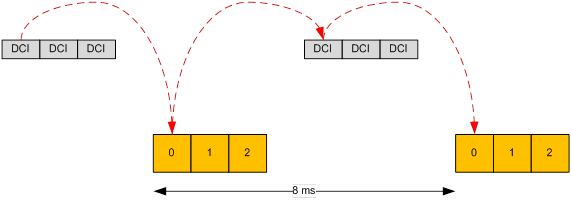
\includegraphics[height=40mm,width=80mm]{harq_timing.png}}
\caption{HARQ timing}
\label{fig_harq_timing}
\end{figure}


The scheduler needs to take care of the timing relationship if multiple HARQ process is involved. As an example, The following lists a few key constraints that to be considered during system design:
•	MPDCCH and PDSCH cannot be sent at the same TTI unless they are using the partial PRBs within the same narrowband.
•	There is one TTI interval between receiving MPDCCH and receiving PDSCH.
•	When MPDCCH, PDSCH or PUSCH is in the middle of transmission (repetition), this device is not eligible for another transmission.
•	When a Cat-M UE sends feedback (ACK/NACK) on PUSCH/PUCCH, this UE is not eligible to be scheduled to receive on DL MPDCCH or PDSCH channel.

\subsection{MPDCCH}
In legacy LTE, the maximum aggregation level (AGL) of PDCCH is 8 while it has been increased to 24 for Cat-M devices. Because the AGL is larger, the number of grants that can be supported per TTI is smaller. Thus, there is a tradeoff of coverage of MPDCCH and the number of grants can be sent per TTI. At an AGL of 24, one narrowband of PDCCH can only support 1 Cat-M device. As both PDSCH and PUSCH transmissions need grants, this means that when we need to support an AGL of 24 in the system, only one user can be served in a given TTI, either in the uplink or downlink direction  .
\subsection{Link adaptation and power control}
As illustrated in [6], the traffic pattern of Cat-M is very unique in the sense that Cat-M devices wake up very infrequently and then send/receive a very small amount of data. As such, Cat-M devices are expected to wake from RRC IDLE state when new data arrives and as a result it is very difficult for any link adaptation or power control mechanism to work as there is no time for convergence given the small amount of data that will be transmitted over the air..  Therefore, the initial modulation and coding scheme (MCS) selection becomes very important. The initial MCS can be selected based on the reported CQI on RACH message 5 for DL or channel estimated based on received  RACH message 3 for UL. Note that if the traffic pattern of Cat-M devices changes, the system should be designed so that link adaptation and power control will improve performance. For example, transmission of VoIP on Cat-M devices is currently being discussed in standards community, and in this case the Cat-M devices may benefit from both link adaptation and power control.

\section{Results}
	In this section, we present some sample simulation results aimed at providing insight into how system design and configuration can affect performance of MTC devices.

\subsection{Assumptions}
We focus here on the use case where MTC devices are being served using the Cat.M1 feature support in LTE. Further it is assumed here that 1.4MHz bandwidth that is allocated is at a fixed location. Table below lists some of key assumptions that are applicable to the results discussed.
Table 3 Assumptions for simulation results
Parameter 	Assumption
Frequency Bands, Macro inter-site distance (ISD)
	2GHz, 500m
Macro-UE Path Loss / Shadow Model	3GPP case 1, PL = 128.1 + 37.6 log10(d\_km)
Shadow fading std. dev = 8 dB
Cat-M UE traffic	1000 bits, mean reading time = 10s with minimum reading time = 2.5 seconds, Dormancy timer = 2 seconds
Fading Channel Profile	ETU 3km/hr for fading generation, but device is stationary.
Macro eNB antenna	17 dBi gain
Vertical pattern: 10 deg. @ 3 dB beamwidth, SLA = 20 dB, ,downtilt =15deg
Body and cable loss	1 dB (data terminal)
Mobile antenna	Omnidirection; -3 dBi gain
eNB Tx power 	2x20W

\subsection{Achievable Rates}
 Take a simple example where eNB sends data to a remote device that is a Cat.M1. The timing relationship is illustrated in the figure below for the single HARQ process where N is repetition size for M-PDCCH, M is the repetition size of PDSCH, Q is the repetition size on PUCCH and P is the processing delay at the eNB.  In this case the achievable rate is roughly 1000/(N+M+Q+P+1+3), where 1 is the interval between MPDCCH and PDSCH, 3 is the interval between PDSCH and PUCCH.
Figure 2 shows the special case of N=4,M=8,Q=4 and P=3 in which case the achievable throughput is around 43kbps. Without any repetition, the throughput would be similar to the legacy case and would be around 100kbps.

\begin{figure}[htbp]
\centerline{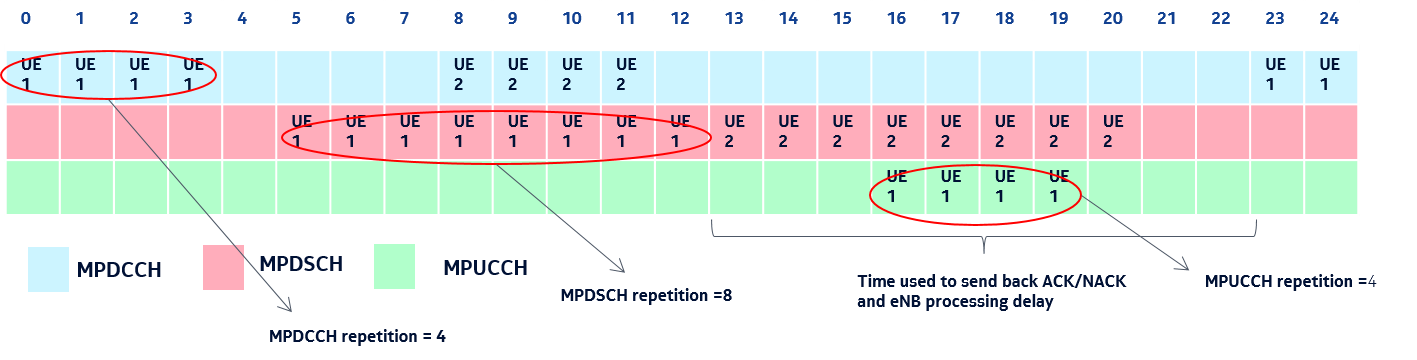
\includegraphics[height=40mm,width=80mm]{timing_relation.png}}
\caption{Illustration of timing relationship between channels}
\label{fig_harq_timing}
\end{figure}


\subsection{Impact of repetition number}
This parameter has significant impact on various performance metrics and some sample results for a single user is shown below. In this plot, we assume the Cat-M traffic as full buffer and focus on the impact of PDSCH repetition number. We assume the repetition numbers of MPDCCH and PUCCH are fixed as 4 and 8, respectively.

\begin{figure}[htbp]
\centerline{\includegraphics[height=60mm,width=80mm]{repetition_impact_on_tp.png}}
\caption{Impact of repetition number on throughput for full buffer}
\label{fig_rep_fb}
\end{figure}



As we can see from the plot in Figure 4, for cell edge users, using a higher repetition size can improve throughput performance. As we discussed in previous sections, increasing the repetition number helps to reduce the number of HARQ retransmission   . In this given configuration, if repetition number of PDSCH =4 , then one HARQ transmission takes N+M+Q+P+4 = 23 TTI. Thus, for three HARQ transmission, it will take 3*23=69 TTI and only 12 (=3*4) repetition of PDSCH packets happens within these 69 TTIs. However, if we use repetition number of  8, each HARQ transmission takes 23+4=27 TTI. And for two HARQ transmission, we can get total of 16 repetitions and the total time used for transmitting these two HARQ transmission is only 2*27 = 54 TTI, which is much smaller than 69 TTI. Certainly, if only one HARQ transmission is needed, then the repetition number is the smaller, the throughput is the higher.
A similar trend can be observed in the burst traffic case as shown in the figure below. Note that in the burst traffic scenario, link adaptation won’t have time to converge.

\begin{figure}[htbp]
\centerline{\includegraphics[height=60mm,width=80mm]{repetition_impact_on_burst_tp.png}}
\caption{Impact of repetition on user traffic for bursty traffic}
\label{fig_rep_burst}
\end{figure}


\subsection{Link Adaptation and power control}
Figures 6A and 6B show sample results on how insensitive uplink performance can be when design choices such as link adaptation and closed power control (CLPC) are considered for a specific traffic profilewhere the average time between packets is in seconds. Due to this the MTC device transmits only 1 measurement and then goes back to “sleep”.  Since there is no convergence in device power from CLPC, the open loop set point is quite important. Figure 6C shows the sensitivity of throughput to the open loop set point.  For the scenario simulated, a lower set point allows multiple PRBs to be used which lowers the code rate and results in improved performance. It should be noted these results do not take into account channel estimation errors which increase as the SINR per PRB is lowered in which case the number of PRBs assigned should be limited to avoid the lower SINR per PRB range.

\begin{figure}[htbp]
\centerline{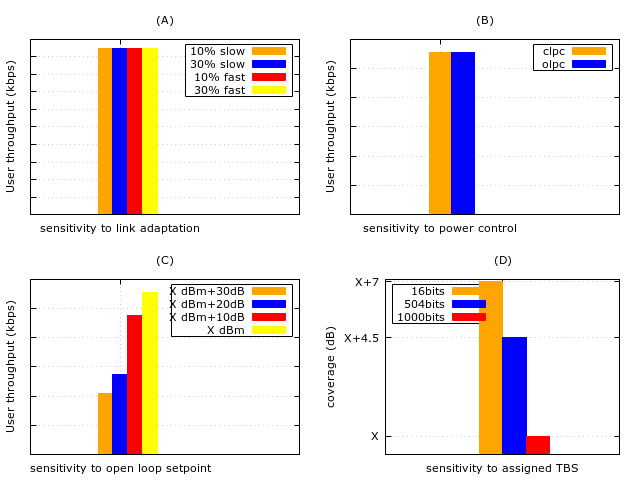
\includegraphics[height=80mm,width=80mm]{sensitivity_to_design.png}}
\caption{MTC performance sensitivity to design parameters (uplink, packet size = 1000bits)}
\label{fig_sensitivity}
\end{figure}



MTC performance sensitivity to design parameters (uplink, packet size = 1000bits)

\subsection{Coverage}
 	Since this is expected to be one of the key metric for MTC devices, maximizing this will drive system design. MTC devices in coverage limited locations are expected to be transmitting at their maximum power. With this resource exhausted, the transport block sizes allocated will impact  coverage . Figure 6D shows the sensitivity of coverage to TBS assignment for a packet size of  1000 bits.  Coverage here is defined as the maximum  path loss at which residual BLER is below 2\%. There is no requirement of latency of packet. It can be seen from the figure that coverage is very sensitive to the TBS assignment. Overall a smaller packet size provides the best coverage performance. This of course comes at the cost of increased latency.
    
\subsection{Latency}
Most MTC applications are not expected to be time critical and latency will be a low priority. For example, a meter that is reporting power consumption at a specific node in a smart grid can tolerate delays on the order of seconds and the key requirement will be reliability.The latency experienced by the report will depend on three key factors:
•	MTC traffic loading
•	Repetition size and/or number of packet segments required to achieve the desired coverage
•	Residual BLER i.e. if the packet does not go through successfully it will require a retransmission
Figure 2 illustrates the latency experienced from the time the scheduler has chosen this packet to be scheduled and initiated a grant transmission of M-PDCCH to the time the feedback (ACK or NACK) has been successfully recived for the packet. The latency (not including latency from layers above the MAC layer) in this case is N+M+P+Q+4 TTIs.  Using a higher repetition size instead of packet segmentation or retransmissions to combat coverage issues might be desirable as in the latter case contention with other MTC devices come into play and impacts latency

\subsection{Interference}
Given that coverage for low cost Cat-M devices is expected to be a key performance metric, interference management will play a key role in being able to meet this requirement. As discussed before, a narrow bandwidth (1.4MHz for Cat.M1 and 200KHz for Cat.NB1) can be reserved for MTC devices. Interference levels in this region are expected to be quite low even though many MTC devices are expected to be supported if this region is not shared with legacy LTE devices. Due to the traffic profile expected for MTC devices, If this region is used to support VoIP traffic, the interference could begin to creep up. In the case that the narrowband resources are shared with legacy LTE devices, interference levels could be quite high and meeting coverage requirements of MTC devices could become more challenging. Therefore a system design consideration could be to consider doing some inter-cell frequency planning to ensure low interference on the reserved MTC narrowbands, which of course comes at the cost of capacity to the legacy LTE devices.

\subsection{VoIP support using MTC devices}
There is an ongoing discussion and studies in 3GPP to understand how VoIP could be supported via Cat-M devices, which may be desirable on wearables for example. While there is expected to be some relaxation on delay budget for the voice traffic packets, latency will still have to be controlled.

\begin{figure}[htbp]
\centerline{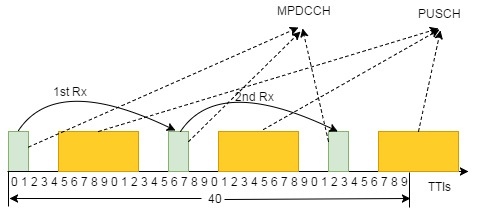
\includegraphics[height=60mm,width=80mm]{voip.png}}
\caption{VoIP scheduling illustration}
\label{fig_voip}
\end{figure}


\subsection{Impact of repetition number on coverage}
Larger repetition number will increase the per link coverage. However, it also results in longer overall time duration for one HARQ transmission. As illustrated in Figure 7, when PUSCH RL=8 and MPDCCH\_RL=2, we can finish two UL HARQ transmission within 40ms. However, when PUSCH RL=16, we will only be able to finish one UL HARQ transmission within 40ms. As VoIP packets arrives with a fixed pattern (every 20ms at talk spurt and 160ms at silent period) and the packets have to be transmitted within a delay budget, larger repetition number means we may have to aggregate more VoIP packets within one HARQ transmission which means a larger TBS. Therefore, we are essentially comparing the two case: higher MCS/TBS with larger repetition number vs. smaller MCS/TBS with smaller repetition number As the gain achieved by the extra repetition may be offset by the loss of the enlarged TBS, increasing the repetition may not necessarily result in larger coverage. For example, table 6 shows that when we increase the PUSCH repetition number from 8 to 16, with the delay budget of 200ms, we see the supported MCL (maximum coupling loss) increasing from 138dB to 140dB. However, when we further increase the repetition from 16 to 32, the MCL even becomes smaller   Thus, there is a balance between increasing the repetition number and TBS increasing.
Table 4 Impact of repetition on coverage
PUSCH repetition	MCL
8	138
16	140
32	138

\subsection{Impact of iBLER selection}
10\% iBLER target is generally used in legacy LTE system for VoIP traffic. In Cat-M systems, as discussed in the previous sections, the HARQ duration is now longer which will result in the collision of HARQ retransmission with the newly arrived voice packets. However, if we lower the iBLER target, for example to 5\%. The HARQ retransmission chance is reduced but it will require more repetitions to support the same TBS at the same SINR. Thus, it is a trade-off between more HARQ vs. repetition  . [7] shows that using HARQ retransmission can achieve higher coverage than without HARQ retransmission (very large repetition). And the best combination of HARQ retransmission number (thus iBLER target) and the repetition number needs more study.

\subsection{Impact of SID packets}
In typical conversational voice scenario, there are two users talking to each other. Even assuming no cross-talk, during a talk spurt of a user, there will be silence insertion descriptor (SID) packets sent from the other user. Thus, this user has voice packet to transmit and at the same time has SID packets to receive. In legacy VoLTE, this is not a big issue due to full duplexing . However, for Cat-M devices, due to the constraints of half duplexing, this user can’t transmit voip packet and receive SID at the same time. Thus, some of the sub frames have to be used for SID receiving which leaves less number of subframes available for UL voip packets transmission. This makes the VoIP scheduling more challenging. For example, one direct impact is that we can’t use the same fixed TBS for VoIP packets anymore as SID happens less frequent compared with voice packets. Whenever SID packets arrives, more aggregation of voice packets will happen.

\subsection{Impact of Segmentation}
Segmentation is generally used in legacy VoLTE to extend the coverage. However, in the case of Cat-M, due to the timing constraints caused by half duplexing, it is challenging to transmit multiple HARQ process at the same time especially when we use larger repetition numbers (as illustrated in figure 2). Assume we only support one HARQ process, and one HARQ duration is 15ms (1+3+8+3 = 15 ms) with the assumption of MPDCCH repetition level of 1 and PUSCH repetition level of 8. Thus, every 20ms, there is only enough time to transmit one HARQ. If we segment a VoIP packets into multiple small segments, the coverage for each segment becomes better but the overall delay could be large.

\section{Conclusions}
We have outlined the numerous system design aspects which must be considered to successfully deploy an LTE network supporting Cat-M MTC devices. The numerous constraints as well as additional coverage/power-saving features the 3GPP standard has included for such devices poses significant challenges integrating support for such devices in an LTE network while minimizing the KPI impact to existing smartphone and other high performance data-centric devices. It has been shown that careful selection of system parameters such as the Cat-M dormancy timer, the number of HARQ transmissions and repetition factor used for Cat-M data and control channels, and the configuration needed to support VoIP on Cat-M devices involves many different tradeoffs, particularly between coverage and latency and also the capacity impact to the legacy LTE network. We have demonstrated that link adaptation features such as closed loop rate conrol and closed loop power control need to be revisited based on the nature of MTC traffic, and certain system settings such as the open loop power control setpoint and default initial MCS assignment become much more critical. It is important to highlight such considerations so that an operator can tailor the parameters and scheduler design aspects to achieve the desired trade-offs inherent in introducing MTC devices into an existing LTE network.



% An example of a floating figure using the graphicx package.
% Note that \label must occur AFTER (or within) \caption.
% For figures, \caption should occur after the \includegraphics.
% Note that IEEEtran v1.7 and later has special internal code that
% is designed to preserve the operation of \label within \caption
% even when the captionsoff option is in effect. However, because
% of issues like this, it may be the safest practice to put all your
% \label just after \caption rather than within \caption{}.
%
% Reminder: the "draftcls" or "draftclsnofoot", not "draft", class
% option should be used if it is desired that the figures are to be
% displayed while in draft mode.
%
%\begin{figure}[!t]
%\centering
%\includegraphics[width=2.5in]{myfigure}
% where an .eps filename suffix will be assumed under latex, 
% and a .pdf suffix will be assumed for pdflatex; or what has been declared
% via \DeclareGraphicsExtensions.
%\caption{Simulation results for the network.}
%\label{fig_sim}
%\end{figure}

% Note that the IEEE typically puts floats only at the top, even when this
% results in a large percentage of a column being occupied by floats.


% An example of a double column floating figure using two subfigures.
% (The subfig.sty package must be loaded for this to work.)
% The subfigure \label commands are set within each subfloat command,
% and the \label for the overall figure must come after \caption.
% \hfil is used as a separator to get equal spacing.
% Watch out that the combined width of all the subfigures on a 
% line do not exceed the text width or a line break will occur.
%
%\begin{figure*}[!t]
%\centering
%\subfloat[Case I]{\includegraphics[width=2.5in]{box}%
%\label{fig_first_case}}
%\hfil
%\subfloat[Case II]{\includegraphics[width=2.5in]{box}%
%\label{fig_second_case}}
%\caption{Simulation results for the network.}
%\label{fig_sim}
%\end{figure*}
%
% Note that often IEEE papers with subfigures do not employ subfigure
% captions (using the optional argument to \subfloat[]), but instead will
% reference/describe all of them (a), (b), etc., within the main caption.
% Be aware that for subfig.sty to generate the (a), (b), etc., subfigure
% labels, the optional argument to \subfloat must be present. If a
% subcaption is not desired, just leave its contents blank,
% e.g., \subfloat[].


% An example of a floating table. Note that, for IEEE style tables, the
% \caption command should come BEFORE the table and, given that table
% captions serve much like titles, are usually capitalized except for words
% such as a, an, and, as, at, but, by, for, in, nor, of, on, or, the, to
% and up, which are usually not capitalized unless they are the first or
% last word of the caption. Table text will default to \footnotesize as
% the IEEE normally uses this smaller font for tables.
% The \label must come after \caption as always.
%
%\begin{table}[!t]
%% increase table row spacing, adjust to taste
%\renewcommand{\arraystretch}{1.3}
% if using array.sty, it might be a good idea to tweak the value of
% \extrarowheight as needed to properly center the text within the cells
%\caption{An Example of a Table}
%\label{table_example}
%\centering
%% Some packages, such as MDW tools, offer better commands for making tables
%% than the plain LaTeX2e tabular which is used here.
%\begin{tabular}{|c||c|}
%\hline
%One & Two\\
%\hline
%Three & Four\\
%\hline
%\end{tabular}
%\end{table}


% Note that the IEEE does not put floats in the very first column
% - or typically anywhere on the first page for that matter. Also,
% in-text middle ("here") positioning is typically not used, but it
% is allowed and encouraged for Computer Society conferences (but
% not Computer Society journals). Most IEEE journals/conferences use
% top floats exclusively. 
% Note that, LaTeX2e, unlike IEEE journals/conferences, places
% footnotes above bottom floats. This can be corrected via the
% \fnbelowfloat command of the stfloats package.


% conference papers do not normally have an appendix



% use section* for acknowledgment
%\ifCLASSOPTIONcompsoc
%  % The Computer Society usually uses the plural form
%  \section*{Acknowledgments}
%\else
%  % regular IEEE prefers the singular form
%  \section*{Acknowledgment}
%\fi
%
%
%The authors would like to thank...





% trigger a \newpage just before the given reference
% number - used to balance the columns on the last page
% adjust value as needed - may need to be readjusted if
% the document is modified later
%\IEEEtriggeratref{8}
% The "triggered" command can be changed if desired:
%\IEEEtriggercmd{\enlargethispage{-5in}}

% references section

% can use a bibliography generated by BibTeX as a .bbl file
% BibTeX documentation can be easily obtained at:
% http://mirror.ctan.org/biblio/bibtex/contrib/doc/
% The IEEEtran BibTeX style support page is at:
% http://www.michaelshell.org/tex/ieeetran/bibtex/
%\bibliographystyle{IEEEtran}
% argument is your BibTeX string definitions and bibliography database(s)
%\bibliography{IEEEabrv,../bib/paper}
%
% <OR> manually copy in the resultant .bbl file
% set second argument of \begin to the number of references
% (used to reserve space for the reference number labels box)
\begin{thebibliography}{1}

\bibitem{mach_research}
www.machinaresearch.com

\bibitem{adyson}
Adyson M. Maia, Dario Vieira†, Miguel F. de Castro, Yacine Ghamri-Doudane, \emph{A Mechanism for Uplink Packet Scheduler in LTE Network in the Context of Machine-to-Machine Communication},  Globecom 2014.

\bibitem{alberto}
Alberto Rico-Alvariño, Madhavan Vajapeyam, Hao Xu, Xiaofeng Wang, Yufei Blankenship, Johan Bergman, Tuomas Tirronen, and Emre Yavuz , \emph{An overview of 3GPP enhancements for machine to machine communications}, IEEE Communications magazine, 2016.

\bibitem{jill}
    Jill Jermyn, Roger Piqueras Jovery, Ilona Murynetsy, Mikhail Istominy and Salvatore Stolfo, \emph{Scalability of Machine to Machine systems and theInternet of Things on LTE mobile networks}, IEEE, 2015

\bibitem{erfan}
    Erfan Soltanmohammadi, Kamran Ghavami, Mort Naraghi-Pour, \emph{A Survey of Traffic Issues in Machine-to-Machine Communications over LTE}, IEEE Internet of Things Journal, 2015

\bibitem{36_888}
    36.888, \emph{Study on provision of low-cost Machine-Type Communications (MTC) User Equipments (UEs) based on LTE}, version 12.0.0.


\end{thebibliography}




% that's all folks
\end{document}


